% The commands: three write declarations, repro verify reads them, repro reproduce reruns them.
% Built to fig_commands_v2.pdf:
%   cd paper/figures && pdflatex fig_commands_v2.tex
\documentclass[border=2pt]{standalone}
\usepackage[T1]{fontenc}
\usepackage{times}
\usepackage{tikz}
\usetikzlibrary{arrows.meta,positioning}

\definecolor{planline}{HTML}{9B59B6}
\definecolor{planfill}{HTML}{F5EEF8}
\definecolor{runline}{HTML}{3498DB}
\definecolor{runfill}{HTML}{EBF5FB}
\definecolor{citeline}{HTML}{E67E22}
\definecolor{citefill}{HTML}{FDF2E9}
\definecolor{checkline}{HTML}{27AE60}
\definecolor{checkfill}{HTML}{E9F7EF}
\definecolor{arrow}{HTML}{7F8C8D}

\newcommand{\cmd}[2]{\textcolor{#1line}{\texttt{\bfseries #2}}}
\newcommand{\dtl}[1]{{\footnotesize\textcolor{black!75}{#1}}}

\begin{document}
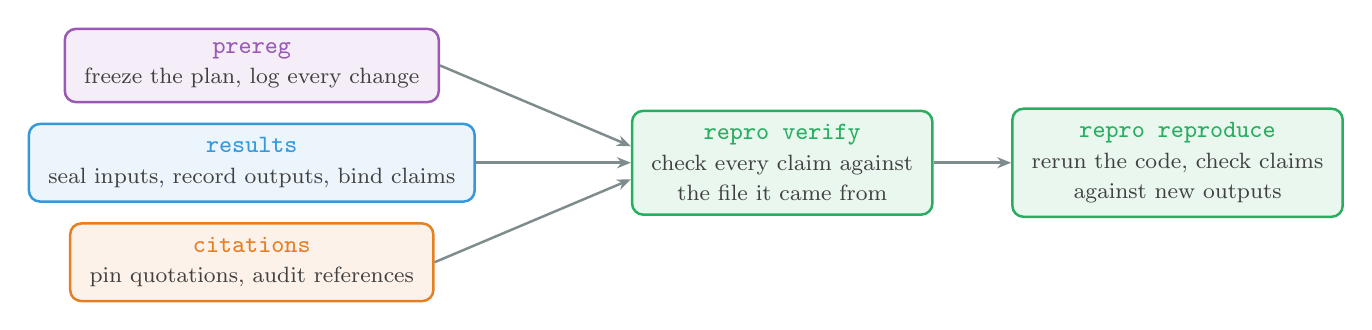
\begin{tikzpicture}[
  command/.style={draw=#1line, fill=#1fill, line width=0.9pt, rounded corners=4pt,
    align=center, inner xsep=7pt, inner ysep=5pt, font=\small},
  feeds/.style={-{Stealth[length=5pt,width=4pt]}, draw=arrow, line width=0.9pt},
]
  \node[command=run] (results) {\cmd{run}{results}\\\dtl{seal inputs, record outputs, bind claims}};
  \node[command=plan, above=7pt of results] (prereg) {\cmd{plan}{prereg}\\\dtl{freeze the plan, log every change}};
  \node[command=cite, below=7pt of results] (citations) {\cmd{cite}{citations}\\\dtl{pin quotations, audit references}};
  \node[command=check, right=56pt of results] (verify)
    {\cmd{check}{repro verify}\\\dtl{check every claim against}\\\dtl{the file it came from}};
  \node[command=check, right=28pt of verify] (reproduce)
    {\cmd{check}{repro reproduce}\\\dtl{rerun the code, check claims}\\\dtl{against new outputs}};
  \draw[feeds] (prereg.east) -- ([yshift=6pt]verify.west);
  \draw[feeds] (results.east) -- (verify.west);
  \draw[feeds] (citations.east) -- ([yshift=-6pt]verify.west);
  \draw[feeds] (verify.east) -- (reproduce.west);
\end{tikzpicture}
\end{document}
